\documentclass[final,hyperref={pdfpagelabels=false}]{beamer}

\mode<presentation>
  {
  %  \usetheme{Berlin}
  \usetheme{uclposter}
  \usecolortheme{ucl}

  \setbeamercolor{block body}{bg=white,fg=black}


  }
  \usepackage{times}
  \usepackage{amsmath,amsthm, amssymb, latexsym}
  \boldmath
  \usepackage[english]{babel}
  \usepackage[latin1]{inputenc}
  \usepackage[orientation=landscape,size=a0,scale=1.4,debug]{beamerposter}

  %%%%%%%%%%%%%%%%%%%%%%%%%%%%%%%%%%%%%%%%%%%%%%%%%%%%%%%%%%%%%%%%%%%%%%%%%%%%%%%%%5
  \graphicspath{{figures/}}
  \title[GVHD]{Quantifying the importance of target organ specific interactions in the aetiology of GVHD}
  \author[Winship \& Plagnol]{Claire Winship, many others, Ron Chakraverty, Vincent Plagnol}
  \institute[UGI]{UCL Genetics Institute}
  \date{\today}

  %%%%%%%%%%%%%%%%%%%%%%%%%%%%%%%%%%%%%%%%%%%%%%%%%%%%%%%%%%%%%%%%%%%%%%%%%%%%%%%%%5
  \begin{document}

  \begin{frame}{} 

  \begin{beamercolorbox}{}
    \maketitle
  \end{beamercolorbox}


    \vfill
    \begin{columns}[t]

      \begin{column}{.25\linewidth}
        \begin{block}{Graft versus host disease}
     \begin{itemize}
          \item In malignant pathologies the donor immune system recognises tumour cells as foreign and eradicates them via immunological mechanisms which together are known as the graft vs tumour (GVT) effect
          \item Donor immune cells may also attack normal host tissue resulting in acute graft vs host disease (GVHD)
          \item The skin, liver and gastrointestinal tract are the most common tissues to be damaged in GVHD
          \item GVHD remains one of the most common post-transplant complications and represents a major barrier to the successful application of allo-HSCT
	  \item A major risk factor involved in GVHD pathology is the use of HLA-mismatched, non related donors
          \item Acute GVHD involves alloreactive donor T-cell mediated cytotoxic response to the tissues of the recipient
          \item Tissue damage caused by cytotoxic T cells leads to recruitment of other effector cells including natural killer cells which further increases tissue injury and results in self perpetuating GVHD
          \item Mice represents the primary model animal for pre-clinical studies of GVHD
          \item Mouse models of acute GVHD usually involve a bone marrow transplant (BMT) which is supplemented with varying numbers/types of donor lymphocites into irradiated allogenic recipients who differ from donors in their MHC class 1 and/or class 2 molecules or in minor histocompatibility antigens
          \end{itemize} 
        \end{block}


        \begin{block}{The ImmGen project}
          \begin{itemize}
          \item The primary aim of ImmGen project is to be comprehensive definition of gene expression and regulatory networks in cells of the mouse immune system
          \item Genes are grouped into modules according to similarities in expression profiles 
          \item Immgen coarse modules consist of groups of genes with broadly similar expression profiles while fine modules represent more defined collections of genes with a high degree of similarity in the expression patterns
	  \item By comparing differentially expressed gene sets to ImmGen, it is possible to identify expression level changes of potentially biologically relevant pathways within the data
          \end{itemize}
        \end{block}

      \end{column}


      \begin{column}{.24\linewidth}
        \begin{block}{T-cell expression in multiple minor histocompatibility antigen-mismatched BMT model}
	  {\bf Objective:} In a polyclonal model, evaluate the differences in gene expression of effector T cells found in the lymphoid organs or in the peripheral tissues through the use of MHC1 knock out mice

	  \begin{minipage}{0.45\textwidth}
	    \includegraphics[width=13cm]{/cluster/project8/vyp/Winship_GVHD/claire/results/mhc1_ko/figs/PCA_prettier.pdf}
	  \end{minipage}	  
	  \begin{minipage}{0.45\textwidth}
	    \includegraphics[width=13cm]{/cluster/project8/vyp/Winship_GVHD/claire/results/mhc1_ko/figs/PCA_prettier_outlier_removed.pdf}
	  \end{minipage}	  
	  {\small
          \begin{itemize}
          \item As shown in the left plot, PCA analysis of all samples reveals presence of outlier in the D7 dataset ($TM008_ko4$)
          \item Decision was made to remove this sample for further analysis in the hope of obtaining more reliable and biologically relevant data
          \end{itemize} }
	  \begin{minipage}{0.45\textwidth}
            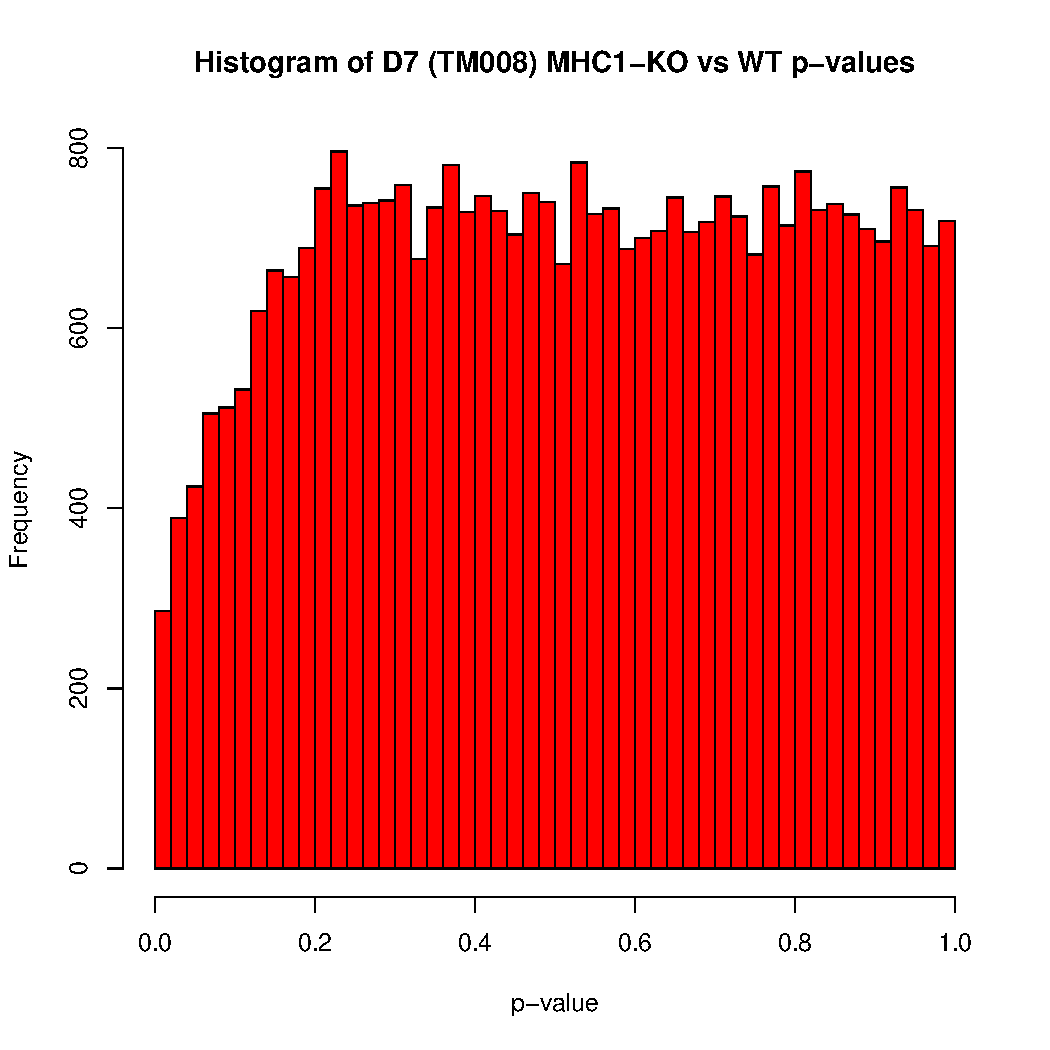
\includegraphics[width=13cm]{/cluster/project8/vyp/Winship_GVHD/claire/results/mhc1_ko/figs/D7_histogram.pdf}
          \end{minipage}
	  \begin{minipage}{0.45\textwidth}
            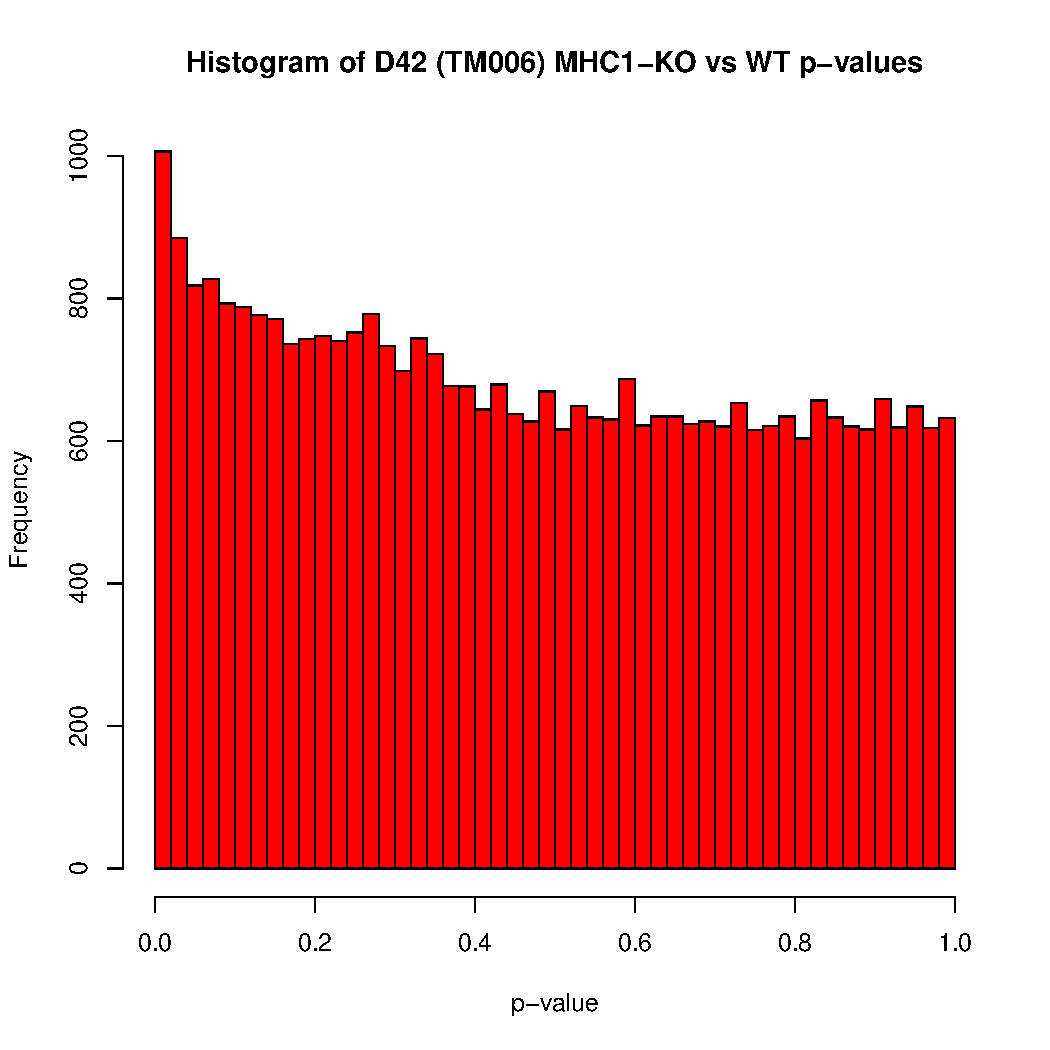
\includegraphics[width=13cm]{/cluster/project8/vyp/Winship_GVHD/claire/results/mhc1_ko/figs/D42_histogram.pdf}
	    \end{minipage}
{\small	  \begin{itemize}
	    \item Histogram of the D7 P-Values does not include outlier sample
	    \item A dip in the plot at low P-Values is visible, this is inconsistent with a uniform distribution of P-Values under the null hypothesis
	    \item The reason for this unusual distribution is still not clear - the RMA package used in this analysis may be a factor but this is currently under investigation 
	\end{itemize}} 
          \begin{minipage}{0.45\textwidth}
            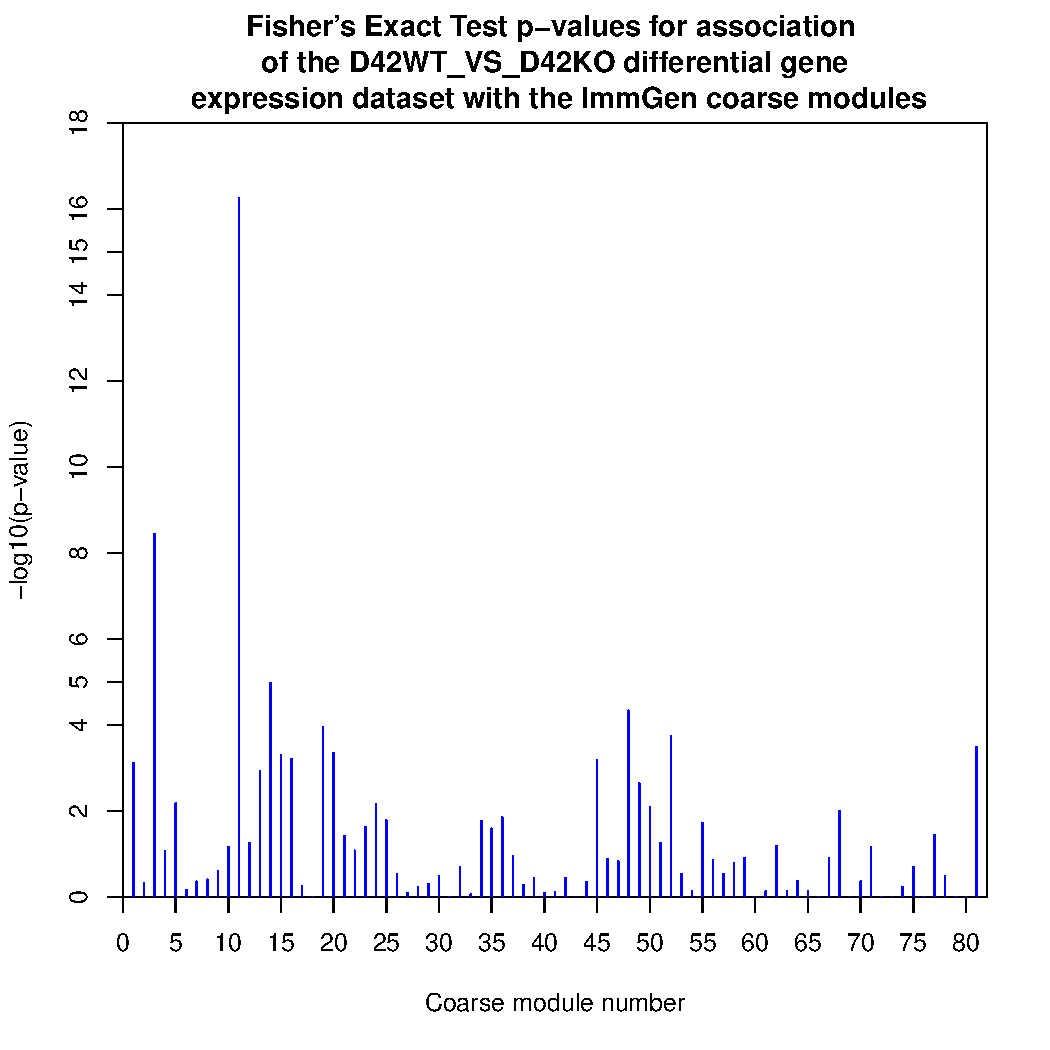
\includegraphics[width=13cm]{/cluster/project8/vyp/Winship_GVHD/claire/results/mhc1_ko/figs/D42WT_VS_D42KO_coarse_module_association_graph.pdf}
          \end{minipage}
          \begin{minipage}{0.45\textwidth}
            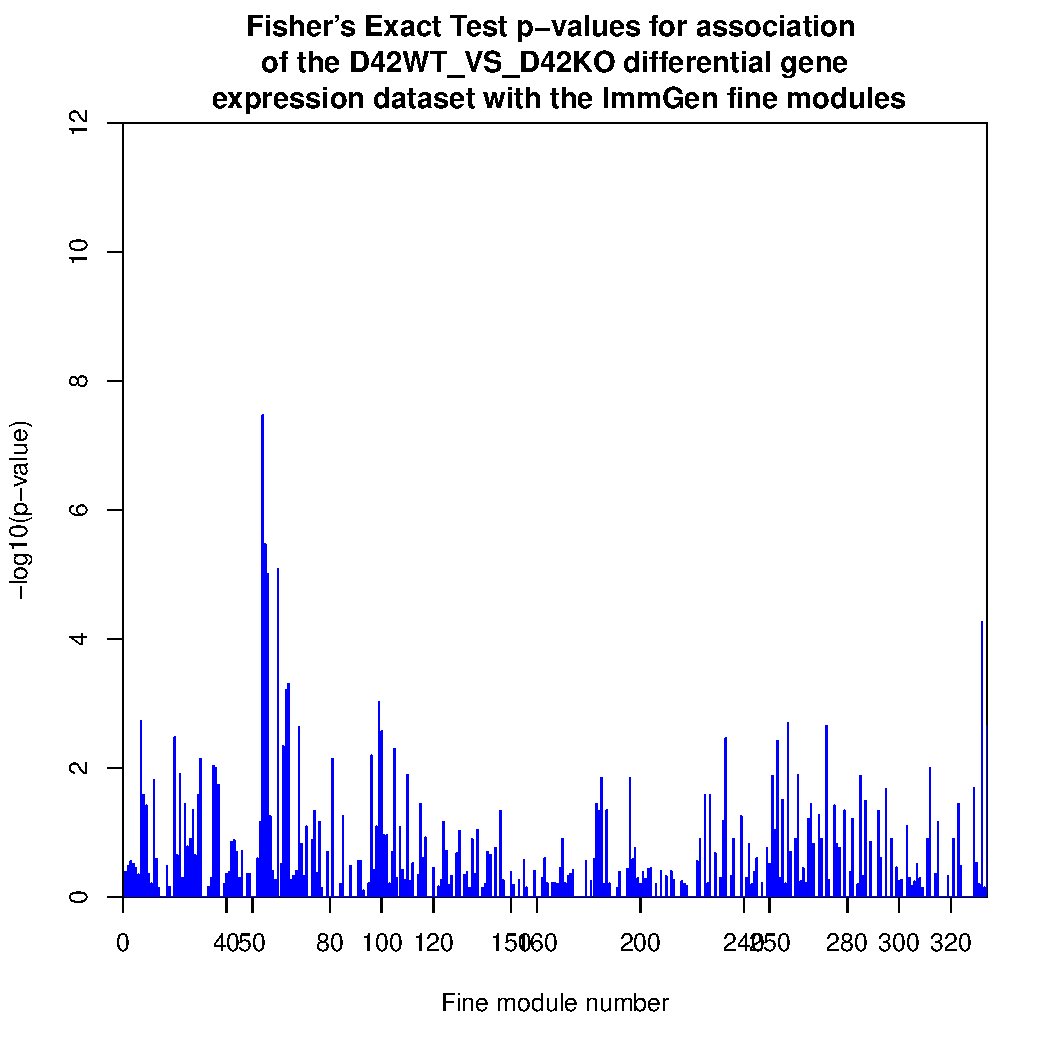
\includegraphics[width=13cm]{/cluster/project8/vyp/Winship_GVHD/claire/results/mhc1_ko/figs/D42WT_VS_D42KO_fine_module_association_graph.pdf}
          \end{minipage}
{\small          \begin{itemize}
            \item Above graphs show the relative associations of the D42 data set with the immgen database, the D7 plots show no significant associations and so are not included here 
            \item Significant associations seen for Coarse module 3 and Fine module 332 
              \end{itemize}}
           %   \begin{minipage}
 	{\scriptsize    \begin{tabular}{ |c|c|c| } 
	    \hline
	    \multicolumn{3}{|c|}{Coarse module 3 most significant differentially expressed genes} \\
	      \hline
	      gene name & fold change & pvalue \\
	      \hline
	      Ptbp2 & 0.8575669378 & 0.0002380649 \\ % The protein encoded by this gene binds to intronic polypyrimidine clusters in pre-mRNA molecules and is implicated in controlling the assembly of other splicing-regulatory proteins.
	      Trappc1 & -0.8105321657 & 0.0011522667 \\ % This gene product plays a role in vesicular transport of proteins to the Golgi apparatus from the endoplasmic reticulum.
	      Mrpl32 & -0.9482075354 & 0.0015174569 \\ % This gene encodes a 39S subunit protein that belongs to the L32 ribosomal protein family. 
	      Ctso & 0.6665616898 & 0.0015502065 \\ % This proteolytic enzyme is involved in cellular protein degradation and turnover. 
	      Cib1 & -0.5435813927 & 0.0022304297 \\ % This gene encodes a member of the EF-hand domain-containing calcium-binding superfamily. The encoded protein interacts with many other proteins, including the platelet integrin alpha-IIb-beta-3, DNA-dependent protein kinase, presenilin-2, focal adhesion kinase, p21 activated kinase, and protein kinase D. The encoded protein may be involved in cell survival and proliferation, and is associated with several disease states including cancer and Alzheimer's disease.
	      Chordc1  & -1.1641319443 & 0.0033252187 \\ % CHORDC1 (Cysteine And Histidine-Rich Domain (CHORD) Containing 1) is a Protein Coding gene. Diseases associated with CHORDC1 include inclusion conjunctivitis. Among its related pathways are Alzheimers disease and Calcineurin-regulated NFAT-dependent transcription in lymphocytes. GO annotations related to this gene include Hsp90 protein binding. An important paralog of this gene is ITGB1BP2.
	      Actr6 & -0.7619741241 & 0.0034636625 \\
	      Pcgf5 & -0.6144202783 & 0.0035618031 \\
	      Llph & -0.797961394 & 0.0047160713 \\
	      1810037I17Rik & -0.6327137658 & 0.0053622021 \\
	      Cd46 & 1.2478436705 & 0.0077584292 \\ % The protein encoded by this gene is a type I membrane protein and is a regulatory part of the complement system. The encoded protein has cofactor activity for inactivation of complement components C3b and C4b by serum factor I, which protects the host cell from damage by complement. 
	      Zfp455 & -1.3221395229 & 0.0083646381 \\ % Zinc finger protein
	      \hline
	    \end{tabular} }
%	\end{minipage}
%	\begin{minipage}
	{\scriptsize    \begin{tabular}{ |c|c|c| } 
	    \hline
	    \multicolumn{3}{|c|}{Fine module 332 differentially expressed genes} \\
	      \hline
	      gene name & fold change & pvalue \\
	      \hline
	      Slc16a6 & 0.4598018044	& 0.012139393 \\ % SLC16A6 (Solute Carrier Family 16, Member 6) is a Protein Coding gene. Diseases associated with SLC16A6 include breast cancer. GO annotations related to this gene include symporter activity and monocarboxylic acid transmembrane transporter activity. An important paralog of this gene is SLC16A11.
		Morc2a	& 0.5233706005	& 0.0128509472 \\ % In humans: Exhibits a cytosolic function in lipogenesis, adipogenic differentiation, and lipid homeostasis by increasing the activity of ACLY, possibly preventing its dephosphorylation. May act as a transcriptional repressor. Down-regulates CA9 expression.
		Cdk2 	& -0.6237586548	& 0.0171621201 \\ % This gene encodes a member of a family of serine/threonine protein kinases that participate in cell cycle regulation. The encoded protein is the catalytic subunit of the cyclin-dependent protein kinase complex, which regulates progression through the cell cycle. 
		St13 	& -0.9037529403 & 0.0178844983 \\ % The protein encoded by this gene is an adaptor protein that mediates the association of the heat shock proteins HSP70 and HSP90. This protein has been shown to be involved in the assembly process of glucocorticoid receptor, which requires the assistance of multiple molecular chaperones. The expression of this gene is reported to be downregulated in colorectal carcinoma tissue suggesting that it is a candidate tumor suppressor gene.
		Dhcr7 	& -0.4962145227	& 0.0184435115 \\
		Hspe1 	& -0.3740957295	& 0.0187365954 \\
		Incenp 	& -0.78546281	& 0.0207810279 \\
	      \hline
	    \end{tabular} }
%	\end{minipage}

        \end{block}
      \end{column}
      \begin{column}{.25\linewidth}
        \begin{block}{T-cell expression: Single minor histocompatibility antigen-mismatched BMT model}
	  {\bf Objective:} In a monoclonal model, evaluate the effect of depleting Langerhans cells on the gene expression of effector T cells found in the lymph nodes and in the skin.
	  \begin{center}
	   \includegraphics[width=15cm]{/cluster/project8/vyp/Winship_GVHD/claire/results/epi_dermis_PLN/figs/PCA_prettier.pdf}
            \end{center}
{\small          \begin{itemize}
          \item some items
          \item some items
          \item some items
          \item some items
          \end{itemize}}
	  \begin{minipage}{0.45\textwidth}
            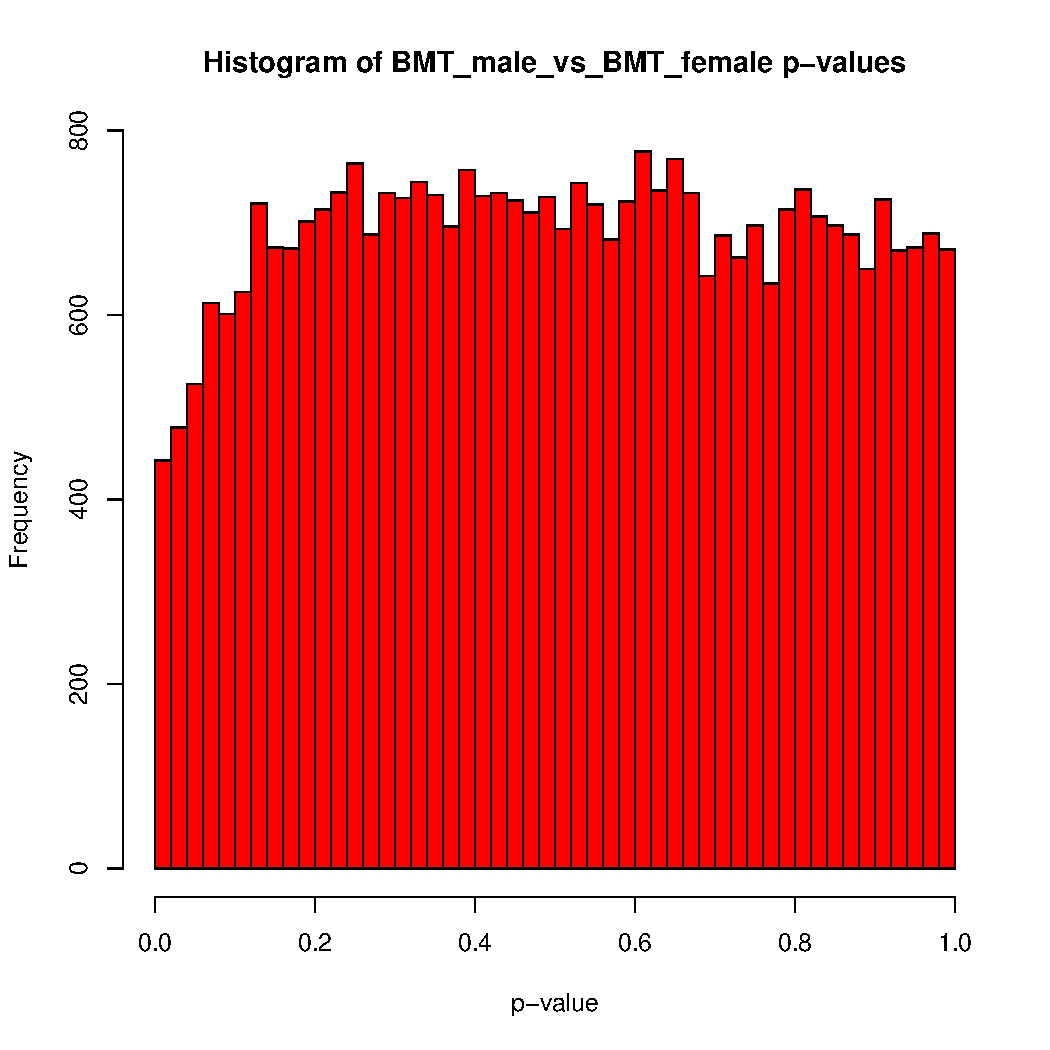
\includegraphics[width=13cm]{/cluster/project8/vyp/Winship_GVHD/claire/results/syn_allo_bmt/figs/BMT_male_vs_BMT_female_histogram.pdf}
          \end{minipage}
          \begin{minipage}{0.45\textwidth}
            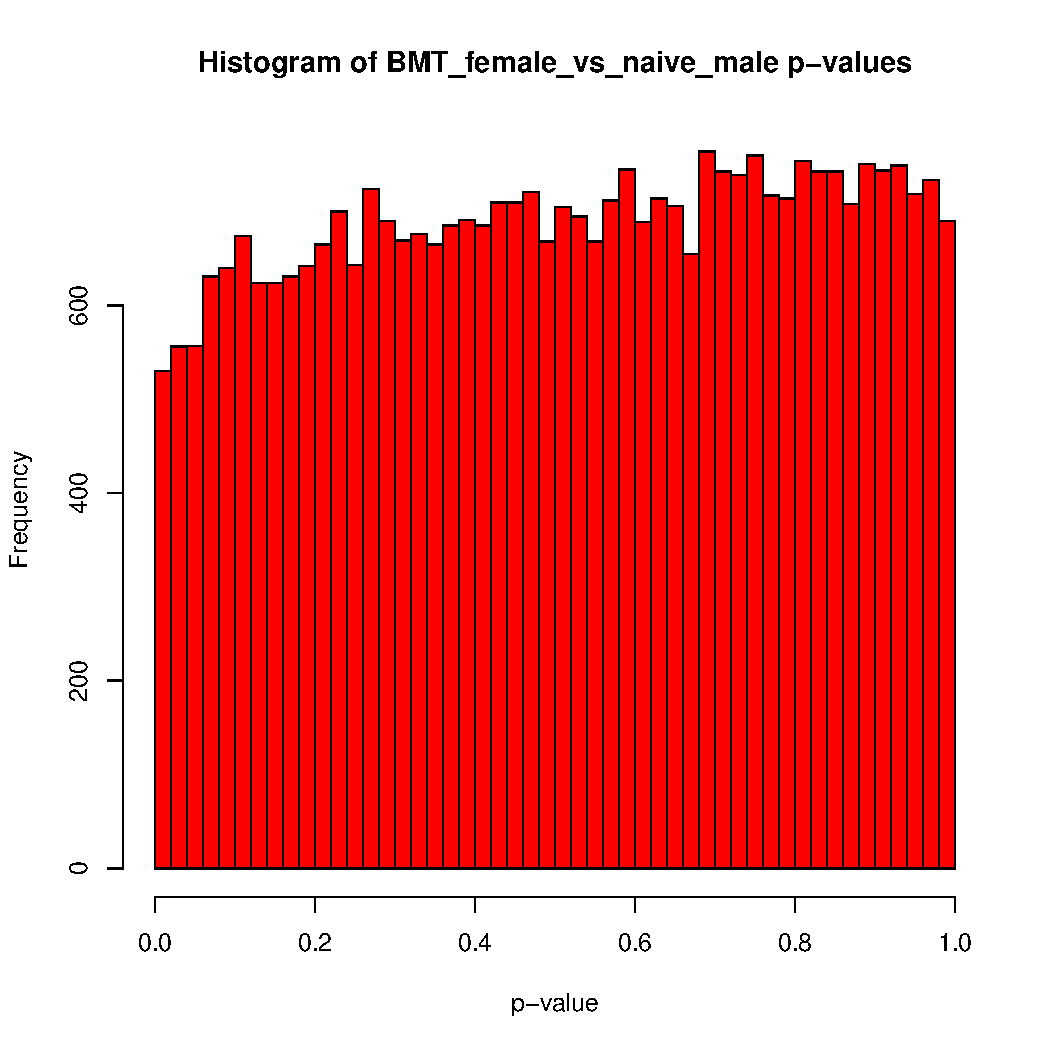
\includegraphics[width=13cm]{/cluster/project8/vyp/Winship_GVHD/claire/results/syn_allo_bmt/figs/BMT_female_vs_naive_male_histogram.pdf}
          \end{minipage}
{\small	  \begin{itemize}
	    \item Histogram of BMT male vs naive male p-values appears to show a more consistent distribution with the null hypothesis 
	    \item some items
	   \end{itemize}}
	  \begin{minipage}{0.45\textwidth}
            \includegraphics[width=13cm]{/cluster/project8/vyp/Winship_GVHD/claire/results/syn_allo_bmt/figs/BMT_male_vs_BMT_female_coarse_module_association_graph.pdf}
            \end{minipage}
{\scriptsize    \begin{tabular}{ |c|c|c| } 
	    \hline
	    \multicolumn{3}{|c|}{Coarse module 34 differentially expressed genes} \\
	      \hline
	      gene name & fold change & pvalue \\
	      \hline
	    
              Gbp5  &	-1.9977876921 &	0.000035098 \\ %GBP5 (Guanylate Binding Protein 5) is a Protein Coding gene. Diseases associated with GBP5 include chronic active epstein-barr virus infection. Among its related pathways are Interferon Signaling and Interferon Signaling. GO annotations related to this gene include identical protein binding and GTPase activity. An important paralog of this gene is GBP7. Human: Stimulates the NLRP3 inflammasome assembly upon bacterial challenge.
              Nlrc5 & 	-1.921796943  &	0.0008103697 \\ %This gene encodes a member of the caspase recruitment domain-containing NLR family. This gene plays a role in cytokine response and antiviral immunity through its inhibition of NF-kappa-B activation and negative regulation of type I interferon signaling pathways.
              Foxp4 &	-1.2158361089 &	0.0218969258 \\
              Clec2D& 	-1.0375138397 &	0.0068116015 \\
              Cblb  &	-0.9141390753 &	0.0055652566 \\
              Tap1  &	-0.8921599554 &	0.0110426477 \\

	      \hline
	    \end{tabular} }
          \begin{minipage}{0.45\textwidth}
            \includegraphics[width=13cm]{/cluster/project8/vyp/Winship_GVHD/claire/results/syn_allo_bmt/figs/BMT_female_vs_naive_male_coarse_module_association_graph.pdf}
          \end{minipage}
{\scriptsize    \begin{tabular}{ |c|c|c| } 
	    \hline
	    \multicolumn{3}{|c|}{Coarse module 11 differentially expressed genes with greatest fold changes} \\
	      \hline
	      gene name & fold change & pvalue \\
	      \hline

Kif11 &	1.2215741328 &	0.0008619543 \\ % This gene encodes a motor protein that belongs to the kinesin-like protein family. Members of this protein family are known to be involved in various kinds of spindle dynamics. The function of this gene product includes chromosome positioning, centrosome separation and establishing a bipolar spindle during cell mitosis.
Cep55 &	1.6438332146 &	0.0001895853 \\ %   % Plays a role in mitotic exit and cytokinesis. Not required for microtubule nucleation. Recruits PDCD6IP and TSG101 to midbody during cytokinesis. 
Ccnb2 &	1.8526622049 &	0.0002459554 \\ %Cyclin B2 is a member of the cyclin family, specifically the B-type cyclins. The B-type cyclins, B1 and B2, associate with p34cdc2 and are essential components of the cell cycle regulatory machinery. B1 and B2 differ in their subcellular localization. Cyclin B1 co-localizes with microtubules, whereas cyclin B2 is primarily associated with the Golgi region. Cyclin B2 also binds to transforming growth factor beta RII and thus cyclin B2/cdc2 may play a key role in transforming growth factor beta-mediated cell cycle control.
Cenpi &	-0.464447851 &	0.0191009403 \\
Spc25 &	0.3327727456 &	0.0383620894 \\

	      \hline
	    \end{tabular} }

	  \begin{minipage}{0.45\textwidth}
            \includegraphics[width=13cm]{/cluster/project8/vyp/Winship_GVHD/claire/results/syn_allo_bmt/figs/BMT_female_vs_naive_male_fine_module_association_graph.pdf}
          \end{minipage}
{\scriptsize    \begin{tabular}{ |c|c|c| } 
	    \hline
	    \multicolumn{3}{|c|}{Fine module 56 differentially expressed genes} \\
	      \hline
	      gene name & fold change & pvalue \\
	      \hline
	    top2a &	2.4866654148 &	2.25401767773146E-005 \\ %This gene encodes a DNA topoisomerase, an enzyme that controls and alters the topologic states of DNA during transcription. This nuclear enzyme is involved in processes such as chromosome condensation, chromatid separation, and the relief of torsional stress that occurs during DNA transcription and replication. It catalyzes the transient breaking and rejoining of two strands of duplex DNA which allows the strands to pass through one another, thus altering the topology of DNA.
Cep55 &	1.6438332146 &	0.0001895853 \\ % Plays a role in mitotic exit and cytokinesis. Not required for microtubule nucleation. Recruits PDCD6IP and TSG101 to midbody during cytokinesis. 
Kif11 &	1.2215741328 &	0.0008619543 \\ % This gene encodes a motor protein that belongs to the kinesin-like protein family. Members of this protein family are known to be involved in various kinds of spindle dynamics. The function of this gene product includes chromosome positioning, centrosome separation and establishing a bipolar spindle during cell mitosis.
Cenpf &	0.7209485514 &	0.0014308153 \\
Anln  &	1.1871751504 &	0.0018927836 \\
              
	      \hline
	    \end{tabular} }
          \begin{minipage}{0.45\textwidth}
            \includegraphics[width=13cm]{/cluster/project8/vyp/Winship_GVHD/claire/results/syn_allo_bmt/figs/BMT_male_vs_naive_male_coarse_module_association_graph.pdf}
          \end{minipage}

{\scriptsize    \begin{tabular}{ |c|c|c| } 
	    \hline
	    \multicolumn{3}{|c|}{Coarse module 34 differentially expressed genes} \\
	      \hline
	      gene name & fold change & pvalue \\
	      \hline
	    Gbp5 	 &-2.3273429132	& 1.50886579665644E-005 \\ % Stimulates the NLRP3 inflammasome assembly upon bacterial challenge. Diseases associated with GBP5 include chronic active epstein-barr virus infection. Among its related pathways are Interferon Signaling and Interferon Signaling.
            Nlrc5 	& -2.0003758767	& 0.000056044 \\ %This gene encodes a member of the caspase recruitment domain-containing NLR family. This gene plays a role in cytokine response and antiviral immunity through its inhibition of NF-kappa-B activation and negative regulation of type I interferon signaling pathways
            Tap1 	& -1.1565143339	& 0.0010494152 \\
            Ly75 	& -1.2495333515	& 0.0016517816 \\
            Samhd1 	& -0.9918372301	& 0.00194126 \\
	      \hline
	    \end{tabular} }
	  \begin{minipage}{0.45\textwidth}
            \includegraphics[width=13cm]{/cluster/project8/vyp/Winship_GVHD/claire/results/syn_allo_bmt/figs/BMT_male_vs_naive_male_fine_module_association_graph.pdf}
          \end{minipage}
        \end{block}
      \end{column}


      \begin{column}{.25\linewidth}
        \begin{block}{Langerhans cell expression}
	  {\bf Objective:} Evaluate the differences in gene expression of Langerhans cells in the setting of an allogeneic BMT or a syngeneic BMT.
           \begin{center}
           \includegraphics[width=15cm]{/cluster/project8/vyp/Winship_GVHD/claire/results/syn_allo_bmt/figs/PCA_prettier.pdf}
          \end{center}
{\small
          \begin{itemize}
          \item some items
          \item some items
          \item some items
          \item some items
          \end{itemize}}

	  \begin{minipage}{0.45\textwidth}
            \includegraphics[width=13cm]{/cluster/project8/vyp/Winship_GVHD/claire/results/epi_dermis_PLN/figs/dermis_vs_dermisDT_histogram.pdf}
          \end{minipage}
          \begin{minipage}{0.45\textwidth}
            \includegraphics[width=13cm]{/cluster/project8/vyp/Winship_GVHD/claire/results/epi_dermis_PLN/figs/epidermis_vs_epidermisDT_histogram.pdf}
          \end{minipage}
          \begin{minipage}{0.45\textwidth}
            \includegraphics[width=13cm]{/cluster/project8/vyp/Winship_GVHD/claire/results/epi_dermis_PLN/figs/PLN_vs_PLNDT_histogram.pdf}
          \end{minipage}
{\small          \begin{itemize}
            \item some items
            \item some items
           \end{itemize}}
	  \begin{minipage}{0.45\textwidth}
            \includegraphics[width=13cm]{/cluster/project8/vyp/Winship_GVHD/claire/results/epi_dermis_PLN/figs/epidermis_vs_epidermisDT_coarse_module_association_graph.pdf}
          \end{minipage}

	  \begin{minipage}{0.45\textwidth}
            \includegraphics[width=13cm]{/cluster/project8/vyp/Winship_GVHD/claire/results/epi_dermis_PLN/figs/epidermis_vs_epidermisDT_fine_module_association_graph.pdf}
          \end{minipage}
{\small	  \begin{itemize}
	    \item some items
	   \end{itemize}}
	  \begin{minipage}{0.45\textwidth}
            \includegraphics[width=13cm]{/cluster/project8/vyp/Winship_GVHD/claire/results/epi_dermis_PLN/figs/PLN_vs_PLNDT_fine_module_association_graph.pdf}
          \end{minipage}


{\small
	  \begin{itemize}
            \item some items
           \end{itemize}}
        \end{block}
      \end{column}


    \end{columns}
  \end{frame}
\end{document}


%%%%%%%%%%%%%%%%%%%%%%%%%%%%%%%%%%%%%%%%%%%%%%%%%%%%%%%%%%%%%%%%%%%%%%%%%%%%%%%%%%%%%%%%%%%%%%%%%%%%
%%% Local Variables: 
%%% mode: latex
%%% TeX-PDF-mode: t
%%% End:
